\documentclass[journal]{IEEEtran}
\input{glyphtounicode}
\pdfgentounicode=1
\usepackage{amsmath,amssymb,bm,booktabs,cite,graphicx}
\renewcommand{\thetable}{S\arabic{table}}
\renewcommand{\thefigure}{S\arabic{figure}}
\renewcommand{\thesection}{S-\Roman{section}}
\renewcommand{\thesectiondis}{S-\Roman{section}}
\newcommand{\Gnn}{\mathcal{G}(n,n)}
\newcommand{\rev}[1]{\widetilde{#1}}
\newcommand{\sgn}{\operatorname{sign}}
\begin{document}
\title{Supplementary Material for\\ ``Geometric Algebra Lifts and Scalar Floquet Criteria\\ for Switched Power Converters''}
\author{Francisco~G.~Montoya and~Alfredo~Alcayde}
\maketitle

Equation, proposition, section, figure and table numbers without the prefix
``S'' refer to the paper.

\section{Proof of Proposition~1}
Write $\bm{u}=\bm{u}_k$, $\bm{n}=\bm{n}_k$, $\sigma=\sigma_k$, $\bm{B}=\bm{B}_k$,
and let $\mathcal{N}=\ker\bm{n}_k^{T}$. From the null lift, $\bm{u}^2=\bm{n}^2=0$
and $2\,\bm{u}\!\cdot\!\bm{n}=\sigma$, hence $\bm{u}\bm{n}+\bm{n}\bm{u}=\sigma$,
$\bm{B}=\bm{u}\bm{n}-\bm{n}\bm{u}$ and $\bm{u}\bm{n}=\tfrac12(\sigma+\bm{B})$,
which is (8). Then
$\bm{B}^2=\bm{u}\bm{n}\bm{u}\bm{n}+\bm{n}\bm{u}\bm{n}\bm{u}
=\sigma\bm{u}\bm{n}+\sigma\bm{n}\bm{u}=\sigma^2$, using
$\bm{u}\bm{n}=\sigma-\bm{n}\bm{u}$ and $\bm{u}^2=\bm{n}^2=0$ repeatedly.

\emph{Spinor norm.} $\rev{\bm{Q}}_S=1+\bm{n}\bm{u}$, so
$\bm{Q}_S\rev{\bm{Q}}_S=1+\bm{u}\bm{n}+\bm{n}\bm{u}+\bm{u}\bm{n}\bm{n}\bm{u}
=1+\sigma$.

\emph{Action.} Let $\bm{x}\in V_w$ and $c=\bm{n}_k^{T}\bm{x}=2\,\bm{n}\!\cdot\!\bm{x}$.
Since $V_w$ is totally null, $\bm{u}\bm{x}=-\bm{x}\bm{u}$, and
$\bm{n}\bm{x}=-\bm{x}\bm{n}+c$. Hence
$\bm{Q}_S\bm{x}=\bm{x}+\bm{u}\bm{n}\bm{x}=\bm{x}+\bm{u}(c-\bm{x}\bm{n})
=\bm{x}+c\,\bm{u}+\bm{x}\bm{u}\bm{n}=\bm{x}\bm{Q}_S+c\,\bm{u}$. For
$1+\sigma\neq0$, $\bm{Q}_S^{-1}=\rev{\bm{Q}}_S/(1+\sigma)$ and
$\bm{u}\rev{\bm{Q}}_S=\bm{u}+\bm{u}\bm{n}\bm{u}=\bm{u}+(\sigma-\bm{n}\bm{u})\bm{u}
=(1+\sigma)\bm{u}$, so $\bm{u}\bm{Q}_S^{-1}=\bm{u}$ and
\begin{equation*}
\bm{Q}_S\bm{x}\bm{Q}_S^{-1}=\bm{x}+c\,\bm{u}\bm{Q}_S^{-1}
=\bm{x}+\bm{u}_k(\bm{n}_k^{T}\bm{x})=S_k\bm{x}.
\end{equation*}
The lift is even and lies in $\operatorname{span}\{1,\bm{B}\}$, the plane
algebra of the blade $\bm{B}$; it fixes the lifts of $\mathcal{N}$ pointwise
because they anticommute with both $\bm{u}$ and $\bm{n}$ and hence commute
with $\bm{u}\bm{n}$.

\emph{Types.} For $\sigma\neq0$ set $\hat{\bm{B}}=\bm{B}/\sigma$, so
$\hat{\bm{B}}^2=1$ and $\bm{Q}_S=1+\tfrac12\sigma+\tfrac12\sigma\hat{\bm{B}}$.
If $1+\sigma>0$, with $\lambda=\ln(1+\sigma)$,
$\sqrt{1+\sigma}\,[\cosh(\lambda/2)+\sinh(\lambda/2)\hat{\bm{B}}]
=\tfrac12(2+\sigma)+\tfrac12\sigma\hat{\bm{B}}=\bm{Q}_S$, which is case (i);
for $\sigma=0$, $\bm{Q}_S=1+\tfrac12\bm{B}$ with $\bm{B}^2=0$. If
$1+\sigma<0$, with $\lambda=\ln\lvert1+\sigma\rvert$,
$\sqrt{\lvert1+\sigma\rvert}\,[\sinh(\lambda/2)+\cosh(\lambda/2)\hat{\bm{B}}]
=-\tfrac12(2+\sigma)-\tfrac12\sigma\hat{\bm{B}}=-\bm{Q}_S$, which is
(9); here $\hat{\bm{B}}$ is itself a versor, since with
$\bm{a}=\bm{u}+\bm{n}$ and $\bm{b}=\bm{u}-\bm{n}$ (invertible, $\bm{a}^2=\sigma$,
$\bm{b}^2=-\sigma$) one has $\bm{a}\bm{b}=-\bm{B}$ and
$\hat{\bm{B}}=(-\bm{a}/\sigma)\bm{b}$, and
$\hat{\bm{B}}\rev{\hat{\bm{B}}}=-\hat{\bm{B}}^2=-1$. If $1+\sigma=0$,
$\bm{Q}_S^2=1+2\bm{u}\bm{n}+\bm{u}\bm{n}\bm{u}\bm{n}=1+(2+\sigma)\bm{u}\bm{n}
=\bm{Q}_S$ and $S_k^2=I+(2+\sigma)\bm{u}_k\bm{n}_k^{T}=S_k$ with $\det S_k=0$.
Finally, the spinor norm is multiplicative: for versors $\bm{W}_1,\bm{W}_2$
with scalar $\bm{W}_i\rev{\bm{W}}_i$,
$(\bm{W}_1\bm{W}_2)\rev{(\bm{W}_1\bm{W}_2)}=\bm{W}_1(\bm{W}_2\rev{\bm{W}}_2)\rev{\bm{W}}_1
=(\bm{W}_1\rev{\bm{W}}_1)(\bm{W}_2\rev{\bm{W}}_2)$, which is the versor half
of Proposition~2. All identities were verified numerically
for generic non-axis-aligned $\bm{u}_k$, $\bm{n}_k$ in $\mathcal{G}(3,3)$ and
$\mathcal{G}(4,4)$ to machine precision (scripts of Section~S-VIII).

\section{Proof of Proposition~3}
Let $a_i^{\dagger}$ and $a_i$ denote exterior multiplication by $e_i$ and
contraction with $e_i$ on $\Lambda\mathbb{R}^{n}$. They satisfy
$a_ia_j^{\dagger}+a_j^{\dagger}a_i=\delta_{ij}$ and
$a_ia_j+a_ja_i=a_i^{\dagger}a_j^{\dagger}+a_j^{\dagger}a_i^{\dagger}=0$, which
are the Witt relations of $\{\bm{w}_i,\bm{v}_j\}$ with the normalization
$\bm{w}_i\!\cdot\!\bm{v}_j=\tfrac12\delta_{ij}$; the map
$\bm{w}_i\mapsto a_i^{\dagger}$, $\bm{v}_i\mapsto a_i$ therefore extends to
an isomorphism $\Gnn\cong\operatorname{End}(\Lambda\mathbb{R}^{n})$, the Fock
representation \cite{lounesto2001}, under which $\bm{w}_i$ acting on the
vacuum gives $e_i\in\Lambda^{1}$ and the scalar part of an element is
$2^{-n}$ of its trace, every other basis blade being traceless. By (6),
$\bm{B}_A/2=\sum_{ij}A_{ij}\bm{w}_i\bm{v}_j-\tfrac12\operatorname{tr}A$, so
$\bm{Q}_{\Phi}=e^{\operatorname{tr}(A\tau)/2}e^{\bm{B}_{A\tau}/2}
=\exp\bigl(\sum_{ij}(A\tau)_{ij}a_i^{\dagger}a_j\bigr)=\Lambda(e^{A\tau})$,
the exterior-power extension of the flow, since the exponential of the
bilinear operator $\sum_{ij}A_{ij}a_i^{\dagger}a_j$ acts on $\Lambda^{k}$ as
$\Lambda^{k}e^{A}$. Likewise
$\bm{Q}_S=1+\sum_{ij}(\bm{u}_k)_i(\bm{n}_k)_j a_i^{\dagger}a_j$ acts on
$e_{j_1}\wedge\dots\wedge e_{j_k}$ by replacing one factor at a time by its
image under $\bm{u}_k\bm{n}_k^{T}$, and terms with two replacements vanish
because $\bm{u}_k\wedge\bm{u}_k=0$; this is $\Lambda^{k}(I+\bm{u}_k\bm{n}_k^{T})$.
Since $\Lambda$ is multiplicative, $\bm{Q}_M=\Lambda(M)$, and
$\operatorname{Tr}\Lambda(M)=\sum_k\operatorname{tr}\Lambda^{k}M=\det(I+M)$, the first identity of (14);
$\bm{Q}_M\rev{\bm{Q}}_M=\det M$ follows from the multiplicativity of the
spinor norm and its values $e^{\operatorname{tr}A\tau}$ and $1+\sigma_k$ on
the factors. The element
$\bm{\Gamma}=\prod_i\bm{e}^{+}_i\bm{e}^{-}_i=\prod_i(1-2\bm{w}_i\bm{v}_i)$ is
$\prod_i(1-2a_i^{\dagger}a_i)=(-1)^{N}$, $N$ the number operator, i.e.\
$(-1)^{k}$ on $\Lambda^{k}$, so
$2^{n}\langle\bm{Q}_M\bm{\Gamma}\rangle_0=\sum_k(-1)^{k}\operatorname{tr}\Lambda^{k}M
=\det(I-M)$, and $\bm{H}(z)=\prod_i[\tfrac12(1+z)+\tfrac12(1-z)(1-2a_i^{\dagger}a_i)]
=z^{N}$ gives (15). All three identities are polynomial in the
entries of $M$ and hold for singular $M$. For $n=2$, $\det(I\pm M)=1\pm\operatorname{tr}M+\det M$,
and $\lvert\det M\rvert<1$, $1\pm\operatorname{tr}M+\det M>0$ are the
Schur--Cohn conditions for both roots of $z^2-(\operatorname{tr}M)z+\det M$
to lie inside the unit circle. The identities were verified numerically for
$n=2,3,4$ with random flows and saltations of every type (scripts of Section~S-VIII).

\section{Cost and Accuracy of the Versor Representations}
The dimension $4^{n}$ of $\Gnn$ is the size of a general multivector. The
lift of a monodromy matrix is a particular element, and its cost depends on
the representation that is adopted. Five routes are compared in
Table~\ref{tab:coste} for a cycle with two events and three intervals.
1) In a generic implementation a multivector is a dense array of $4^{n}$
coefficients and a product uses the Cayley table, with $16^{n}$
multiplications. 2) In the spinor (Fock) representation of Section~S-II a
multivector is a $2^{n}\times2^{n}$ matrix and a product costs $8^{n}$
multiplications. 3) The lift of an element of $GL(n,\mathbb{R})$ preserves
the grade in that representation. It is therefore block diagonal, with one
block $\Lambda^{k}M$ of size $\binom{n}{k}$ per grade, and a product costs
$\sum_k\binom{n}{k}^{3}$ multiplications. 4) A versor is a product of
vectors and can be stored as the list of its factors in the
$2n$-dimensional space. A composition is a concatenation, a saltation with
$\sigma_k\neq0$ contributes the two factors $\bm{u}_k+\bm{n}_k$ and
$\bm{u}_k/\sigma_k+(1+1/\sigma_k)\bm{n}_k$, and the action on a vector is a
chain of reflections. The count of Table~\ref{tab:coste} assumes the
Cartan--Dieudonn\'e bound of $2n$ factors per interval flow. 5) The matrix
route uses $n\times n$ products and rank-one updates. The first three
routes grow exponentially with $n$, whereas the factored versor is within a
constant factor of about ten of the matrix route. The three structured
representations were verified against the element $1+\bm{u}\bm{n}$ and
against the matrix identities of Proposition~3 to $3\times10^{-15}$ for
$n=2$, $3$ and $4$.

\begin{table}[!h]
\caption{Multiplications Required by Each Representation. Routes 1--3 and
the Matrix Product: One Product of Two Lifts. Factored Versor and Matrix
Cycle: Complete Cycle With Two Events and Three Intervals.}
\label{tab:coste}
\centering
\footnotesize
\setlength{\tabcolsep}{3pt}
\begin{tabular}{@{}rrrrrrrr@{}}
\toprule
 & \multicolumn{4}{c}{one product} & \multicolumn{3}{c}{complete cycle} \\
\cmidrule(lr){2-5}\cmidrule(l){6-8}
$n$ & generic & spinor & blocks & $n\times n$ & factored & matrix & ratio \\
\midrule
2 & $256$ & $64$ & $10$ & $8$ & $320$ & $32$ & $10.0$ \\
3 & $4096$ & $512$ & $56$ & $27$ & $924$ & $90$ & $10.3$ \\
4 & $6.6\times10^{4}$ & $4096$ & $346$ & $64$ & $2016$ & $192$ & $10.5$ \\
5 & $1.0\times10^{6}$ & $3.3\times10^{4}$ & $2252$ & $125$ & $3740$ & $350$ & $10.7$ \\
6 & $1.7\times10^{7}$ & $2.6\times10^{5}$ & $1.5\times10^{4}$ & $216$ & $6240$ & $576$ & $10.8$ \\
7 & $2.7\times10^{8}$ & $2.1\times10^{6}$ & $1.0\times10^{5}$ & $343$ & $9660$ & $882$ & $11.0$ \\
8 & $4.3\times10^{9}$ & $1.7\times10^{7}$ & $7.4\times10^{5}$ & $512$ & $14144$ & $1280$ & $11.1$ \\
\bottomrule
\end{tabular}
\end{table}

The factored representation is the one implemented by the numerical library
of \cite{eid2025gafl}, in which a versor of a quadratic space of arbitrary
signature is stored as a matrix of reflection normals and a scaling factor.
The cycle of Table~\ref{tab:coste} was built with that library in the
signature $(n,n)$ with a null basis, and compared with the matrix route in
the same runtime (.NET~10) over $30$ random cycles per order.
Table~\ref{tab:tiempos} reports the results. The interval rotors are
factored by the library into $4n-2$ reflections, above the bound assumed in
Table~\ref{tab:coste}, and the composition is a concatenation. The factored
versor reproduced the monodromy matrix within $1.2\times10^{-14}$ for
$n\le7$ and $8\times10^{-13}$ for $n=8$, and the sign of $\det M$ obtained
from the signs of the squares of the factors was correct in the $210$
cycles. The matrix route is faster by a factor that grows from $3$ to $12$
for the composition and from $9$ to $55$ for the action on a vector. At
these sizes the times of the matrix route are dominated by call overhead,
and the ratios are indicative.

\begin{table}[!h]
\caption{Measured Times With the Library of \cite{eid2025gafl}: Composition
of the Cycle and Action on One Vector (Microseconds).}
\label{tab:tiempos}
\centering
\footnotesize
\setlength{\tabcolsep}{4pt}
\begin{tabular}{@{}rrrrrrr@{}}
\toprule
 & & & \multicolumn{2}{c}{composition} & \multicolumn{2}{c}{action} \\
\cmidrule(lr){4-5}\cmidrule(l){6-7}
$n$ & factors & error of $M$ & versor & matrix & versor & matrix \\
\midrule
2 & 22 & $3.1\times10^{-15}$ & $2.7$ & $0.90$ & $0.87$ & $0.09$ \\
3 & 34 & $5.9\times10^{-15}$ & $5.2$ & $0.91$ & $1.68$ & $0.10$ \\
4 & 46 & $1.2\times10^{-14}$ & $8.7$ & $1.12$ & $2.74$ & $0.12$ \\
5 & 58 & $6.9\times10^{-15}$ & $11.9$ & $1.31$ & $3.76$ & $0.12$ \\
6 & 70 & $7.6\times10^{-15}$ & $17.2$ & $1.69$ & $5.72$ & $0.14$ \\
7 & 82 & $9.6\times10^{-15}$ & $23.1$ & $2.10$ & $8.10$ & $0.17$ \\
8 & 94 & $8.0\times10^{-13}$ & $26.6$ & $2.30$ & $9.66$ & $0.18$ \\
\bottomrule
\end{tabular}
\end{table}

Table~\ref{tab:condic} reports the accuracy near the three degeneracies of
the event types for $n=4$ and three events, the second of which is driven
toward the degeneracy. The reference is the matrix product, and each entry
is a median over $16$ random cycles. Three implementations are compared.
The first is the generic multivector implementation used in the first
version of the paper, with the normalized versor, for which medians over
eight instances are available at four points. The second is the factored
versor composed by concatenation. The third is the same factored versor
after it is assembled into the $2n\times2n$ matrix of its action and
factored again, which is the composition performed by the MATLAB port of
the library when the number of factors exceeds the dimension. The factored
versor maintains an error of about $3\times10^{-15}$ over twenty decades of
$\lvert1+\sigma\rvert$ and down to $\lvert\sigma\rvert=10^{-10}$. Beyond
these values one factor is a null vector within the tolerance of the
library, and the construction is rejected. The assembled matrix contains
both $M$ and its inverse transpose. The entries of the latter grow as the
event approaches the singular type, and the second factorization loses the
digits and, from $\lvert1+\sigma\rvert=10^{-8}$, the sign in $5$ of $16$
cycles. For comparison, an LU factorization of the assembled $n\times n$
product recovers $\sgn\det M$ down to $\lvert1+\sigma\rvert=10^{-13}$.

\begin{table}[!h]
\caption{Relative Error of the Monodromy Matrix Near the Degenerate Event
Types ($n=4$, Three Events, the Second One Degenerating). ---: Not
Evaluated.}
\label{tab:condic}
\centering
\footnotesize
\setlength{\tabcolsep}{3pt}
\begin{tabular}{@{}llccc@{}}
\toprule
limit & value & generic, & factored, & assembled and \\
 & & normalized & concatenated & factored again \\
\midrule
singular & $\lvert1+\sigma\rvert=10^{-2}$ & --- & $2.9\times10^{-15}$ & $3.1\times10^{-12}$ \\
 & $10^{-4}$ & $6\times10^{-10}$ & $2.8\times10^{-15}$ & $1.5\times10^{-7}$ \\
 & $10^{-6}$ & --- & $2.8\times10^{-15}$ & $3.8\times10^{-4}$ \\
 & $10^{-8}$ & $5\times10^{-6}$ & $2.9\times10^{-15}$ & $1.8$ \\
 & $10^{-10}$ & --- & $3.6\times10^{-15}$ & $1.0$ \\
 & $10^{-12}$ & --- & rejected & rejected \\
\addlinespace[2pt]
grazing & $\lvert1+\sigma\rvert=10^{2}$ & --- & $2.8\times10^{-15}$ & $8.4\times10^{-12}$ \\
 & $10^{4}$ & --- & $3.0\times10^{-15}$ & $5.5\times10^{-8}$ \\
 & $10^{6}$ & --- & $2.8\times10^{-15}$ & $8.5\times10^{-4}$ \\
 & $10^{8}$ & --- & $3.0\times10^{-15}$ & $1.5$ \\
 & $10^{10}$ & $4.5\times10^{-6}$ & $2.7\times10^{-15}$ & $0.98$ \\
\addlinespace[2pt]
parabolic & $\sigma=10^{-2}$ & --- & $4.2\times10^{-15}$ & $1.5\times10^{-14}$ \\
 & $10^{-6}$ & --- & $2.9\times10^{-15}$ & $1.4\times10^{-10}$ \\
 & $10^{-10}$ & --- & $3.2\times10^{-15}$ & $1.7\times10^{-15}$ \\
 & $10^{-12}$ & --- & rejected & rejected \\
\bottomrule
\end{tabular}
\end{table}

A time-triggered event has $\sigma=0$ exactly. Its plane contains no
invertible vector, and the event is not a product of two vectors of that
plane; it is kept in the form $1+\bm{u}\bm{n}$ of (8).

\section{Sensing Dynamics and the Reflection Count}
Table~\ref{tab:sensado} reports the experiment of Section~V-G in which a
first-order current-sensing filter with corner frequency $f_f$ is placed
ahead of the comparator of the platform of Section~V-A, at $m_a=50$~kA/s.
The state is $[i_L,v_C,i_f]^{T}$ with $\dot i_f=2\pi f_f(i_L-i_f)$, and the
switching function is $h=i_f-(I_{\mathrm{ref}}-m_at)$. With ideal sensing
the event is of reflection type, $1+\sigma=-0.5259$, and the multipliers are
$-0.5205$ and $0.9660$. With the filter, $\det S=1$ and $N_r=0$ in every
row, and the product of the two slow multipliers is negative. The third
multiplier, obtained from (12) and the two slow ones, is real and negative.
The last column indicates whether the sign of $\det M$ obtained from an LU
factorization of the assembled matrix is correct. It fails at
$f_f=50/T$, where the determinant is of order $10^{-137}$, whereas the sum
of the rapidities and the count are exact in every row.

\begin{table}[!h]
\caption{Buck Converter of Section~V-A With a First-Order Current-Sensing
Filter ($m_a=50$~kA/s).}
\label{tab:sensado}
\centering
\footnotesize
\setlength{\tabcolsep}{3pt}
\begin{tabular}{@{}rrrrrrc@{}}
\toprule
$f_fT$ & $1+\sigma$ & $\ln\lvert\det M\rvert$ & flip & voltage & fast & LU sign \\
\midrule
$0.5$ & $1$ & $-3.19$ & $-0.4932$ & $0.9641$ & $-8.7\times10^{-2}$ & correct \\
$1$ & $1$ & $-6.33$ & $-0.5563$ & $0.9647$ & $-3.3\times10^{-3}$ & correct \\
$2$ & $1$ & $-12.61$ & $-0.5351$ & $0.9653$ & $-6.5\times10^{-6}$ & correct \\
$5$ & $1$ & $-31.46$ & $-0.5263$ & $0.9657$ & $-4.3\times10^{-14}$ & correct \\
$8$ & $1$ & $-50.31$ & $-0.5241$ & $0.9658$ & $-2.8\times10^{-22}$ & correct \\
$12$ & $1$ & $-75.44$ & $-0.5229$ & $0.9659$ & $-3.4\times10^{-33}$ & correct \\
$20$ & $1$ & $-125.71$ & $-0.5219$ & $0.9659$ & $-5.0\times10^{-55}$ & correct \\
$50$ & $1$ & $-314.20$ & $-0.5210$ & $0.9660$ & $-6.9\times10^{-137}$ & wrong \\
\bottomrule
\end{tabular}
\end{table}

\section{Hybrid Differential-Algebraic Example: Numerical Details}
The following details complete the discussion of \cite{hayes2020application}
in Section~V-H. Under maximum-power-point tracking the
switching function involves only the algebraic variable, so $\bm{n}_x=0$;
discarding $\bm{n}_y$, as an ODE treatment does, leaves $\tilde{\bm{n}}=0$
and hence $S=I$. From their published transition matrices,
$\det\Phi_{\mathrm{on}}\det\Phi_{\mathrm{off}}=0.7430$ at $R=37\,\Omega$,
while the multipliers they report for that treatment, $0.8505\pm0.1436j$,
give $\det M=0.7440$, a ratio of $1.0014$: approximately consistent with
$S=I$ and $N_r=0$, the residual being an internal discrepancy of the
published data (their printed matrices return the pair $0.8506\pm0.1397j$).
Proposition~2 then forbids a forced real negative
multiplier, and none appears; the ODE treatment cannot see the period
doubling that the circuit undergoes. With (22) restored, their
multipliers become $0.7533$ and $-0.993$, so $\det S=-1.0068$: a reflection
event, $N_r=1$, and the flip channel opens. At $R=37.1\,\Omega$ the same
computation gives $\det S=-1.0358$ and the negative multiplier crosses $-1$.
The discrepancy between the two treatments, which \cite{hayes2020application}
identifies and resolves by deriving the corrected saltation, is in the
present language a change of type caused by the wrong covector; the
covector formulation explains why the correction had to take the form it
did.

\section{Simultaneous Events: Plant and Randomized Search}
This section gives the complete account that is summarized in Section~V-J.
When two events coincide, the order of the corresponding factors in
(1) is no longer fixed by the dynamics and there are two
candidate monodromies. For given saltation matrices the order changes $M$
and its spectrum (over $400$ random pairs of reflection-type saltations in
$n=4$, by a median $129\%$ of the monodromy's magnitude) but not $\det M$,
the total rapidity or $\bm{W}\rev{\bm{W}}$, which are one identity,
$\det(S_aS_b)=\det(S_bS_a)$, in three forms. The ambiguity lives in the
commutator, which the dictionary gives as
$[\bm{B}_a,\bm{B}_b]=2\bm{B}_{[S_a,S_b]}$. In matrix terms
$S_aS_b-S_bS_a=\alpha\,\bm{u}_a\bm{n}_b^{T}-\beta\,\bm{u}_b\bm{n}_a^{T}$ with
$\alpha=\bm{n}_a^{T}\bm{u}_b$ and $\beta=\bm{n}_b^{T}\bm{u}_a$, a matrix of
rank at most two, and $\operatorname{tr}(S_aS_b)=n+\sigma_a+\sigma_b+\alpha\beta$,
so the interference between two saltations is the coordinate-free scalar
$\alpha\beta$.

The physical question is harder, because the saltations must then be
rebuilt in each order: the intermediate vector field differs, so
$\dot h^{+}/\dot h^{-}$ need not be the same number. Two identical buck
modules in parallel on a common output ($C=220\,\mu$F, $R=2\,\Omega$,
$I_{\mathrm{ref}}=2.6$~A, no compensation ramp, $D\approx0.87$; the
period-one orbit is itself unstable, which the construction permits), with
the same clock and the same peak reference, give the benign answer. Without
magnetic coupling $\bm{u}_1$ has no component in phase~2 nor conversely, so
$\bm{n}_1^{T}\bm{u}_2=\bm{n}_2^{T}\bm{u}_1=0$, the two saltations commute, and
the corner is removable. Coupling the inductors destroys the commutation,
and breaking the symmetry between the phases as well ($L_2/L_1=1.6$,
$k=0.5$, phase-2 reference $2.566$~A) makes $\det M$ order-dependent,
$5.505$ against $22.010$. Sweeping the mismatch through zero confirms that
this is not an artifact of how the corner is assembled: the true monodromy
converges to one candidate from the left and to the other from the right
(Fig.~\ref{fig:esquina}), so $\det M$ has a finite jump at the corner
although every event is transversal on both sides. The budget
(12) remains exact on each branch; what the corner removes is a
unique derivative of the cycle map \cite{dibernardo2001corner,burden2016}.

\begin{figure}[!h]
\centering
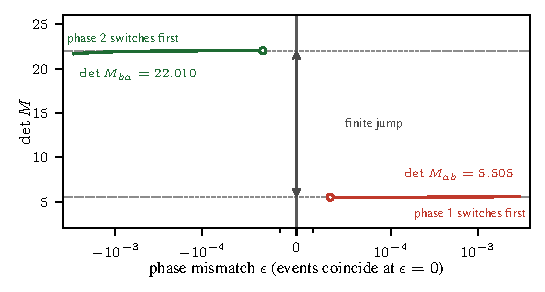
\includegraphics[width=\columnwidth]{figs/esquina_simultanea.pdf}
\caption{Simultaneous events. Two magnetically coupled, unequal phases
whose turn-offs collide at $\epsilon=0$. The monodromy converges to a
different candidate from each side, so that $\det M$ drops by $75\%$ across
the corner, and the budget (12) by $\ln4$, although every event is
transversal on both sides. Here the sign is preserved. In one of the $1029$
admissible corners that were sampled it is not.}
\label{fig:esquina}
\end{figure}

Whether the sign can depend on the order as well is a sharper question,
because a solution of the periodicity and threshold conditions is not
automatically an orbit of the latch: it must also start each cycle with both
comparators below their references and reach the corner before either
trips. A randomized search over $3000$ coupled, mismatched pairs produced
$1269$ solutions of the periodicity and threshold conditions, $1029$ of
which passed a $199$-point guard screen along the on--on segment, and
exactly one in which $N_r$ depends on the order ($k=0.91$, $L_2/L_1=1.20$,
$R_2/R_1=1.17$, $R=1.33\,\Omega$, phase references $2.7200$ and $2.1959$~A,
$D=0.562$). Both separated-event continuations exist around it, with
$\det M\to+50.1$ from one side and $\to-0.0013$ from the other. The products
of the two saltation determinants are $-0.00147$ in one order and $+57.6$
in the other, and the near-singular factor can be named: in the order in
which phase~1 switches first, the phase-2 saltation has
$\det S=1.17\times10^{-4}$, with an outgoing crossing velocity of $70$~A/s
against an incoming $6\times10^{5}$~A/s. The ambiguity therefore arises next
to the singular type boundary of Proposition~1, not away
from it. The mechanism is that switching one phase alters the current slope
of the other, so the type of the second event depends on whether the
first has already occurred. Both orders are transversal, and
(13) returns the correct sign for each; what is not defined at
a coupled simultaneous corner is the count $N_r$ itself. This is why
Proposition~2 carries the separation hypothesis, and it
delimits the result: strongly coupled converters must be checked for event
coincidence before the count is read off the schematic.

\section{Randomized Verification Ensemble and Excluded Data}
The ensemble of Section~V-H contains $2\times10^{4}$ random
switched systems with $n=2,\dots,8$, up to six rank-one factors per period,
random interval matrices $A_i$ with entries of order $0.7/\sqrt{n}$, interval
durations in $[0.05,1]$, and event types drawn across the classification with
$\lvert1+\sigma_k\rvert\ge0.05$. Trials with $\operatorname{cond}M\ge10^{10}$
(224 of them, $1.1\%$) were excluded before the eigenvalue comparison. In the
remaining $19\,776$ systems the sign of $\det M$ from the closed form
$\exp(\sum_i\operatorname{tr}(A_i)\tau_i)\prod_k(1+\sigma_k)$, from the
assembled product, and from the parity of the real negative multipliers
agreed in every case; the worst relative discrepancy between the closed form
and the assembled determinant was $6.3\times10^{-7}$. In $4\,891$ trials
($24\%$ of the ensemble) an even $N_r$ came with two or more real negative
multipliers. In addition, in $200$ systems in
$\mathcal{G}(2,2)$--$\mathcal{G}(4,4)$ with $\bm{u}_k$ and $\bm{n}_k$ drawn at
random, the generic multivector implementation reproduced the monodromy to a
relative $5.7\times10^{-11}$.

One published study was examined and left out of Table~V. The two negative
multipliers reported for a two-stage power-factor corrector in
\cite{wang2012period} belong to an averaged line-frequency model without
switching events, in which Liouville's formula already fixes the sign.

\section{The Even Case: Derivation and Simulation Data}
This section derives (19)--(21) and the closed form of $\chi_k$, and reports
the data that are summarized in Section~V-D.

\emph{Reduction.} The state of the two-phase converter is
$\bm{x}=[i_1,i_2,v_C]^{T}$. With $\gamma=R/(R+r_C)$, the interval matrix
is, in every configuration,
\begin{equation*}
A=\begin{bmatrix}-r_1&-e_1&-a_1\\-e_2&-r_2&-a_2\\c&c&-g\end{bmatrix},
\quad
\begin{aligned}
e_k&=\gamma r_C/L_k,& a_k&=\gamma/L_k,\\
c&=\gamma/C,& g&=\gamma/(RC),
\end{aligned}
\end{equation*}
where $r_k$ is the series resistance of phase $k$ divided by $L_k$, plus
$e_k$. Only $r_k$ depends on the configuration. The turn-off of phase $k$
modifies the $k$th component of the vector field only, so that
$S_k=I+\sigma_k\bm{e}_k\bm{e}_k^{T}$. If the period is started immediately
after the event of phase~2, the monodromy matrix is similar to
$S_2\Phi''S_1\Phi'$, where $\Phi'$ and $\Phi''$ are the flows between the
events. With equal duty cycles each of them has the duration $h=T/2$ and,
to the order that is retained, the blocks
\begin{equation*}
\Phi_{cc}=\begin{bmatrix}1-\rho_1'&-\eta_1\\-\eta_2&1-\rho_2'\end{bmatrix},\;\;
\Phi_{cv}=-\begin{bmatrix}\beta_1\\\beta_2\end{bmatrix},\;\;
\Phi_{vc}=\zeta\,[\,1\ \,1\,],
\end{equation*}
with $\eta_k=e_kh+\tfrac12\beta_k\zeta$, $\beta_k=a_kh$, $\zeta=ch$,
$\rho_k'=\int r_k\,dt+\tfrac12\beta_k\zeta$ and $\Phi_{vv}\approx1$. The
term $e_kh$ is the direct interaction through the ESR, and
$\tfrac12\beta_k\zeta$ is the interaction through the capacitor voltage. The
two flip multipliers are close to $d=1+\sigma$ and far from the voltage
multiplier, which is close to unity. The voltage can therefore be eliminated
by the Schur complement of the product evaluated at $\mu=d$,
$M_{\mathrm{eff}}=M_{cc}+M_{cv}M_{vc}/(d-1)$. To leading order,
\begin{equation*}
\begin{gathered}
M_{\mathrm{eff}}=\begin{bmatrix}\mu_1+s_1&\chi_1\\d\,\chi_2&\mu_2+s_2\end{bmatrix},\\
\chi_k=-(1+d)\,e_kh-\beta_k\zeta\,\frac{d^{2}+6d+1}{2(d-1)},
\end{gathered}
\end{equation*}
where $\mu_k=(1+\sigma_k)e^{-\rho_k}$, $\rho_k$ is the integral of the series
resistance of phase $k$ divided by $L_k$ over one period, and
$s_k=2\beta_k\zeta\,d(1+d)/(1-d)$. With $d=-e^{\lambda}$, where $\lambda=\ln\lvert1+\sigma\rvert$ is the rapidity
of the two events, and $\beta_k\zeta=\gamma^{2}T^{2}/(4L_kC)$, the expression
of $\chi_k$ becomes
\begin{equation}
\chi_k=-\frac{\gamma Te^{\lambda/2}}{2L_k}\left[\frac{\gamma T}{4C}\,
\frac{3-\cosh\lambda}{\cosh(\lambda/2)}-2r_C\sinh\frac{\lambda}{2}\right],
\tag{S1}
\end{equation}
and $s_k=\gamma^{2}T^{2}e^{\lambda}\tanh(\lambda/2)/(2L_kC)$. The shift
$s_k$ is common to both phases for equal inductances and vanishes at
$\lambda=0$. It displaces the center of the pair, by about $-6\times10^{-4}$ at
the operating point of Table~III, and it is omitted in (19) and (20). The
eigenvalues of $M_{\mathrm{eff}}$ are (20) with $\chi^{2}=-d\,\chi_1\chi_2$,
and at $\lambda=0$ the bracket of (S1) reduces to $\gamma T/(2C)$, which
gives (21).

\emph{Closed form against the monodromy matrix.} Table~\ref{tab:chi}
compares (S1) with the value of $\chi$ that is obtained from the Schur
complement of the monodromy matrix for equal phases. In the $45$ points that
were evaluated ($C=47$, $100$ and $220\,\mu$F, $r_C=0$, $25$ and
$50$~m$\Omega$, $\lvert1+\sigma\rvert$ from $0.34$ to $0.93$) the largest
deviation is $7.0\%$, at $C=47\,\mu$F, $r_C=0$ and $\lvert1+\sigma\rvert=0.34$,
and it does not exceed $1.6\%$ for $\lvert1+\sigma\rvert\ge0.65$. At the stability
boundary with the ramp of $10$~kA/s, (21) gives $2.419\times10^{-3}$ and the
monodromy matrix $2.404\times10^{-3}$. For $L_2/L_1=1.02$ the mismatch is
$\Delta\mu=-6.257\times10^{-3}$ from the closed form and
$-6.242\times10^{-3}$ from the monodromy matrix, and for
$R_L=60/52$~m$\Omega$ the two values are $-5.256\times10^{-3}$ and
$-5.243\times10^{-3}$, respectively.

\begin{table}[!h]
\caption{Interference $\chi$ for Equal Phases: Closed Form (S1) and
Monodromy Matrix ($m_a=0$).}
\label{tab:chi}
\centering
\footnotesize
\setlength{\tabcolsep}{4pt}
\begin{tabular}{@{}rrrccr@{}}
\toprule
$C$ [$\mu$F] & $r_C$ [m$\Omega$] & $\lvert1+\sigma\rvert$ & monodromy & closed form & deviation \\
\midrule
47 & 25 & 0.659 & $3.553\times10^{-3}$ & $3.514\times10^{-3}$ & $-1.1\%$ \\
47 & 25 & 0.933 & $4.836\times10^{-3}$ & $4.874\times10^{-3}$ & $+0.8\%$ \\
100 & 0 & 0.659 & $1.545\times10^{-3}$ & $1.541\times10^{-3}$ & $-0.3\%$ \\
100 & 0 & 0.933 & $2.313\times10^{-3}$ & $2.329\times10^{-3}$ & $+0.7\%$ \\
100 & 25 & 0.343 & $9.780\times10^{-4}$ & $9.704\times10^{-4}$ & $-0.8\%$ \\
100 & 25 & 0.659 & $1.828\times10^{-3}$ & $1.832\times10^{-3}$ & $+0.2\%$ \\
100 & 25 & 0.933 & $2.311\times10^{-3}$ & $2.333\times10^{-3}$ & $+0.9\%$ \\
100 & 50 & 0.659 & $2.101\times10^{-3}$ & $2.114\times10^{-3}$ & $+0.6\%$ \\
220 & 25 & 0.659 & $1.010\times10^{-3}$ & $1.018\times10^{-3}$ & $+0.8\%$ \\
220 & 25 & 0.933 & $1.092\times10^{-3}$ & $1.104\times10^{-3}$ & $+1.1\%$ \\
\bottomrule
\end{tabular}
\end{table}

\emph{Event type and direction of the separation.} Table~\ref{tab:tipo}
reports the pair of the converter with equal phases while the ramp is raised
beyond the deadbeat slope, so that both events change from reflection to
pass-through. With two reflections the pair is complex, and with two
pass-through events it consists of two real multipliers, as the sign of
$\chi^{2}=-d\,\chi_1\chi_2$ requires. With pass-through events the closed form
underestimates the separation by $7\%$ to $12\%$.

\begin{table}[!h]
\caption{Separation of the Pair Across the Deadbeat Slope (Equal Phases,
$D=0.40$). Half-Separation: Imaginary Part for a Complex Pair, Half of the
Difference for a Real Pair.}
\label{tab:tipo}
\centering
\footnotesize
\setlength{\tabcolsep}{3pt}
\begin{tabular}{@{}rrlcc@{}}
\toprule
 & & & \multicolumn{2}{c}{half-separation $[\times10^{-3}]$} \\
\cmidrule(l){4-5}
$m_a$ [kA/s] & $1+\sigma$ & pair (monodromy) & monodromy & closed form \\
\midrule
0 & $-0.6592$ & $-0.6525\pm0.0018j$ & $1.83$ & $1.83$ \\
20 & $-0.3093$ & $-0.3066\pm0.0009j$ & $0.87$ & $0.86$ \\
40 & $-0.0813$ & $-0.0807\pm0.0002j$ & $0.16$ & $0.16$ \\
60 & $+0.0791$ & $+0.0789$, $+0.0785$ & $0.19$ & $0.17$ \\
100 & $+0.2898$ & $+0.2911$, $+0.2873$ & $1.88$ & $1.74$ \\
150 & $+0.4477$ & $+0.4542$, $+0.4439$ & $5.15$ & $4.51$ \\
\bottomrule
\end{tabular}
\end{table}

\emph{Time-domain simulation.} The simulator is event-driven and does not
use saltation matrices. Between events the affine flow is evaluated exactly
from the eigendecomposition of the interval matrix, and each comparator
crossing is located by a safeguarded Newton iteration. The clock of each
phase closes the switch and restarts the ramp, the comparator opens the
switch, and the latch holds it open until the next clock edge. The Jacobian
of the stroboscopic map, obtained by central differences on the simulator,
agrees with the monodromy matrix within $3\times10^{-8}$ at the ten
operating points that were compared, and the pair is complex or real in the
simulator in the same cases. Each run starts on the period-one orbit with an
antisymmetric perturbation of $10^{-6}$~A. The attractor is classified from
the last part of the run with a tolerance of $10^{-9}$~A, and the modulation
frequency is obtained from the spectrum of the even samples.

Table~\ref{tab:umbral} reports the sweep of Fig.~5, with $3\times10^{6}$
cycles per run, of which the last $10^{6}$ are analyzed. Fig.~\ref{fig:series}
shows the inductor current of phase~1 sampled at the clock in two of those
runs. Close to the
threshold the simulated modulation is slower than the value given by the
monodromy matrix, which is the expected behavior of an oscillation of finite
amplitude near the transition. Table~\ref{tab:atractor} reports the
classification for eight mismatches and seven distances from the boundary,
with $6\times10^{5}$ cycles per run. At $50$~mA two of the four cases with
$\lvert\Delta\mu\rvert<2\chi$ have locked to a period-two orbit. In the
period-two regime the subharmonic is concentrated in one phase: for the
mismatch of Table~III, the amplitudes at $1$~mA are $36.1$~mA and $3.5$~mA
in phases~1 and~2, respectively.

\begin{figure}[!h]
\centering
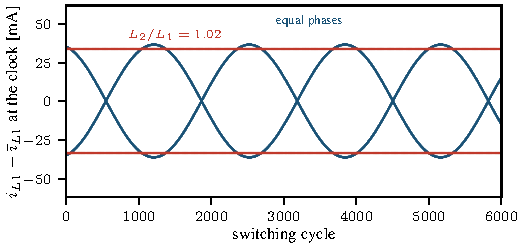
\includegraphics[width=\columnwidth]{figs/par_flip_series.pdf}
\caption{Inductor current of phase~1 sampled at the clock, $1$~mA beyond
the stability boundary ($m_a=10$~kA/s), with the mean value removed. With
equal phases the two subharmonic levels exchange every half modulation
period. With $L_2/L_1=1.02$ the attractor is a period-two orbit.}
\label{fig:series}
\end{figure}

\begin{table}[!h]
\caption{Modulation of the Subharmonic at $1$~mA Beyond the Boundary
($m_a=10$~kA/s, $R_L=60/60$~m$\Omega$). Angle per Cycle
$\theta\ [\times10^{-3}$~rad$]$; M: Modulated Subharmonic; P2: Period-Two
Orbit.}
\label{tab:umbral}
\centering
\footnotesize
\setlength{\tabcolsep}{4pt}
\begin{tabular}{@{}cccccc@{}}
\toprule
$L_2/L_1$ & $\lvert\Delta\mu\rvert/2\chi$ & $\theta$, (20)--(21) & $\theta$, monodromy & $\theta$, simulation & attractor \\
\midrule
1.0000 & 0.000 & 2.419 & 2.400 & 2.386 & M \\
1.0020 & 0.130 & 2.396 & 2.378 & 2.362 & M \\
1.0040 & 0.260 & 2.331 & 2.313 & 2.296 & M \\
1.0060 & 0.390 & 2.220 & 2.202 & 2.183 & M \\
1.0080 & 0.521 & 2.057 & 2.038 & 2.016 & M \\
1.0100 & 0.652 & 1.825 & 1.806 & 1.778 & M \\
1.0120 & 0.783 & 1.496 & 1.475 & 1.438 & M \\
1.0130 & 0.849 & 1.271 & 1.249 & 1.202 & M \\
1.0140 & 0.914 & 0.972 & 0.946 & 0.883 & M \\
1.0145 & 0.947 & 0.769 & 0.738 & 0.656 & M \\
1.0150 & 0.980 & 0.475 & 0.425 & 0.277 & M \\
1.0155 & 1.013 & --- & --- & --- & P2 \\
1.0160 & 1.045 & --- & --- & --- & P2 \\
1.0170 & 1.111 & --- & --- & --- & P2 \\
1.0180 & 1.176 & --- & --- & --- & P2 \\
1.0200 & 1.308 & --- & --- & --- & P2 \\
1.0250 & 1.637 & --- & --- & --- & P2 \\
\bottomrule
\end{tabular}
\end{table}

\begin{table}[!h]
\caption{Attractor Beyond the Stability Boundary ($m_a=10$~kA/s) Against
the Distance $\Delta I_{\mathrm{ref}}$. M: Modulated Subharmonic; P2:
Period-Two Orbit. The Ratio Is That of the Monodromy Matrix at $1$~mA.}
\label{tab:atractor}
\centering
\footnotesize
\setlength{\tabcolsep}{3pt}
\begin{tabular}{@{}lcccccccc@{}}
\toprule
 & & \multicolumn{7}{c}{$\Delta I_{\mathrm{ref}}$ [mA]} \\
\cmidrule(l){3-9}
mismatch & $\lvert\Delta\mu\rvert/2\chi$ & 0.5 & 1 & 2 & 5 & 10 & 20 & 50 \\
\midrule
none & 0.001 & M & M & M & M & M & M & M \\
$L_2/L_1=1.005$ & 0.326 & M & M & M & M & M & M & M \\
$L_2/L_1=1.010$ & 0.654 & M & M & M & M & M & M & P2 \\
$R_L=60/56$~m$\Omega$ & 0.546 & M & M & M & M & M & M & P2 \\
$R_L=60/52$~m$\Omega$ & 1.093 & P2 & P2 & P2 & P2 & P2 & P2 & P2 \\
$L_2/L_1=1.020$ & 1.314 & P2 & P2 & P2 & P2 & P2 & P2 & P2 \\
$L_2/L_1=1.050$ & 3.334 & P2 & P2 & P2 & P2 & P2 & P2 & P2 \\
as in Table~III & 5.147 & P2 & P2 & P2 & P2 & P2 & P2 & P2 \\
\bottomrule
\end{tabular}
\end{table}

\emph{Published multipliers of the two-phase boost converter.}
Table~\ref{tab:giaouris} compares the multipliers listed in Table~I of
\cite{giaouris2013foldings} ($V_{\mathrm{in}}=5$~V, $R=40\,\Omega$,
$L=1.5$~mH, $C=10\,\mu$F, $T=100\,\mu$s, equal phases, no ramp) with those
of the monodromy matrix computed as in Section~II. The values agree within
the four digits printed in four of the five rows. In the row of $0.1$~A the
source prints an imaginary part of $0.0014$ together with a modulus of
$0.1972$. The value computed here, $0.0295$, corresponds to that modulus. In
the row of $0.25$~A the duty cycle obtained here is $0.4124$, which
satisfies the steady-state relation (2) of \cite{giaouris2013foldings},
whereas $0.4367$ is printed. At the boundary the two events have
$1+\sigma=-0.8351$, and the reduction of this section, evaluated
numerically, gives $\chi=0.0367$. Without a ramp, a mismatch of $20\%$ in
the inductance leaves $\lvert\Delta\mu\rvert/2\chi=0.010$. A difference of
$150$~mV between the input voltages of the two phases gives a ratio of
$0.81$ and a complex pair, and a difference of $200$~mV gives $1.04$ and two
real multipliers, $-1.012$ and $-1.036$.

\begin{table}[!h]
\caption{Multipliers of the Two-Phase Boost Converter of
\cite{giaouris2013foldings}: Published and Computed.}
\label{tab:giaouris}
\centering
\footnotesize
\setlength{\tabcolsep}{4pt}
\begin{tabular}{@{}lll@{}}
\toprule
$I_{\mathrm{ref}}$ [A] & published & computed \\
\midrule
0.1 & $0.3132$, $-0.1949\pm0.0014j$ & $0.3132$, $-0.1949\pm0.0295j$ \\
0.25 & $0.5255$, $-0.8324\pm0.0125j$ & $0.5255$, $-0.8324\pm0.0125j$ \\
0.29 & $0.5428$, $-0.9947\pm0.0341j$ & $0.5428$, $-0.9947\pm0.0341j$ \\
0.291166 & $0.5432$, $-0.9994\pm0.0349j$ & $0.5432$, $-0.9994\pm0.0349j$ \\
0.3 & $0.5462$, $-1.0346\pm0.0408j$ & $0.5462$, $-1.0346\pm0.0408j$ \\
\bottomrule
\end{tabular}
\end{table}

\section{Scripts}
All results are reproduced by the scripts of the repository accompanying the
paper. The figures are produced by \texttt{figs/fig0\_geometria.py} to
\texttt{figs/fig5\_par\_flip.py} and \texttt{figs/fig\_tutorial.py}.
The scripts \texttt{figs/verifica\_*.py} check Propositions~1 and~3, every
published number, the complete two-state example and the normal-form
parameters of Section~IV-D
(\texttt{verifica\_ejemplo\_completo.py}), and the energy-metric statement of
Section~VI (\texttt{verifica\_metrica\_energia.py}). The scripts
\texttt{validacion/exp1\_falsacion\_paridad.py} to
\texttt{validacion/exp6\_eventos\_simultaneos.py} cover the ensemble, the
generic-implementation column of Table~\ref{tab:condic}, the deadbeat check,
the fourth-order platform, the digital delay and the simultaneous events.
The scripts added in the revision are \texttt{exp7\_modo\_tension.py}
(voltage-mode buck converter), \texttt{exp8\_boost.py} (boost converter),
\texttt{exp9\_sensado.py} (Table~\ref{tab:sensado}) and
\texttt{exp10\_coste\_representaciones.py} (Table~\ref{tab:coste}). The
folder \texttt{validacion/exp11\_par\_flip/} covers Section~V-D and this
supplement: \texttt{par\_flip\_interleaved.py},
\texttt{par\_flip\_forma\_cerrada.py}, \texttt{par\_flip\_tipo.py} and
\texttt{numeros\_texto.py} (closed form, Tables~\ref{tab:chi}
and~\ref{tab:tipo}), \texttt{sim\_dosfases.py},
\texttt{td1\_validacion.py}, \texttt{td2\_atractor.py} and
\texttt{td3\_umbral.py} (time-domain simulator,
Tables~\ref{tab:umbral} and~\ref{tab:atractor}), and
\texttt{par\_flip\_giaouris.py} (Table~\ref{tab:giaouris}). The
programs of \texttt{validacion/nuga/} produce Table~\ref{tab:tiempos} and
the last two columns of Table~\ref{tab:condic}; they require the library of
\cite{eid2025gafl}. Python 3.9 or later with \texttt{numpy}, \texttt{scipy},
\texttt{numba} and \texttt{clifford} is required, and the figure scripts
render their text with \texttt{pdflatex}.

\begin{thebibliography}{9}
\bibitem{lounesto2001} P. Lounesto, \emph{Clifford Algebras and Spinors},
2nd ed. Cambridge, U.K.: Cambridge Univ. Press, 2001.

\bibitem{eid2025gafl} A. H. Eid, ``GeometricAlgebraFulcrumLib: A unified
generic C\# library for geometric algebra computations,'' GitHub repository,
2025. [Online]. Available:
\texttt{https://github.com/\allowbreak{}ga-explorer/\allowbreak{}GeometricAlgebraFulcrumLib}

\bibitem{hayes2020application} B. Hayes, M. Condon, and D. Giaouris,
``Application of the Filippov method to PV-fed DC--DC converters modeled as
hybrid-DAEs,'' \emph{Eng. Rep.}, vol. 2, no. 9, p. e12237, Sep. 2020,
doi: 10.1002/eng2.12237.

\bibitem{dibernardo2001corner} M. di Bernardo, C. J. Budd, and
A. R. Champneys, ``Corner collision implies border-collision bifurcation,''
\emph{Physica D}, vol. 154, no. 3--4, pp. 171--194, Jun. 2001,
doi: 10.1016/S0167-2789(01)00250-0.

\bibitem{burden2016} S. A. Burden, S. S. Sastry, D. E. Koditschek, and
S. Revzen, ``Event-selected vector field discontinuities yield
piecewise-differentiable flows,'' \emph{SIAM J. Appl. Dyn. Syst.}, vol. 15,
no. 2, pp. 1227--1267, 2016, doi: 10.1137/15M1016588.

\bibitem{wang2012period} F.-Q. Wang, H. Zhang, and X.-K. Ma,
``Period-doubling bifurcation in two-stage power factor correction converters
using the method of incremental harmonic balance and Floquet theory,''
\emph{Chin. Phys. B}, vol. 21, no. 2, p. 020505, Feb. 2012,
doi: 10.1088/1674-1056/21/2/020505.
\bibitem{giaouris2013foldings} D. Giaouris, S. Banerjee, F. Stergiopoulos,
S. Papadopoulou, S. Voutetakis, B. Zahawi, V. Pickert, A. Abusorrah,
M. Al Hindawi, and Y. Al-Turki, ``Foldings and grazings of tori in current
controlled interleaved boost converters,'' \emph{Int. J. Circuit Theory
Appl.}, vol. 42, no. 10, pp. 1080--1091, Oct. 2014, doi: 10.1002/cta.1906.

\end{thebibliography}
\end{document}
